\newcommand{\posterProtonSpin}[2]{

\setlength{\frameWidth}{#1}
\setlength{\frameHeight}{#2}
\setlength{\unitlength}{0.02\frameWidth}
\psset{unit=\unitlength}


\rput[t](44,30){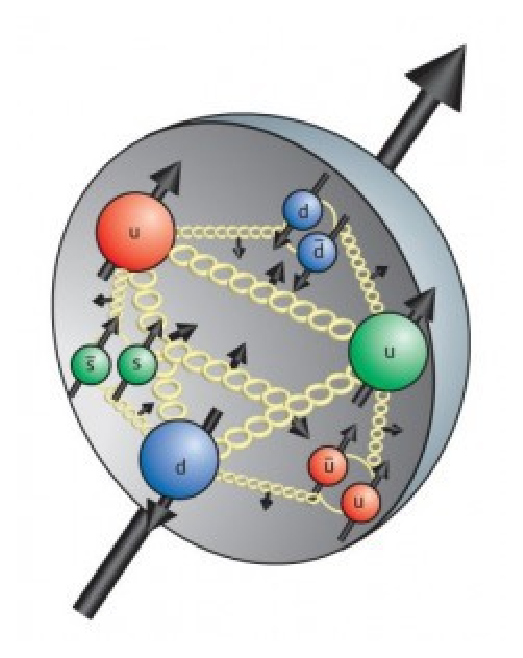
\includegraphics[width=11\unitlength]{graphics/proton}}

\rput[lt](2,29) {%
\begin{minipage}{36\unitlength}

\raggedright

\begin{list}{\labelitemi}{\setlength{\itemsep}{0mm}
                          \setlength{\topsep}{0mm}
                          \setlength{\leftmargin}{0mm}
                          \setlength{\rightmargin}{0mm}}

   \item Proton is a composite particle made of \textbf{quarks and gluons}

   \begin{list}{\labelitemii}{\setlength{\itemsep}{5mm}}

      \item At low interaction energies proton is a point-like particle

      \item At high RHIC energies we see the internal structure of the protons

   \end{list}

\end{list}

\end{minipage}
}

\rput[lt](2,15) {%
\begin{minipage}{46\unitlength}

\begin{list}{\labelitemi}{\setlength{\itemsep}{0mm}
                          \setlength{\topsep}{0mm}
                          \setlength{\leftmargin}{0mm}
                          \setlength{\rightmargin}{0mm}}

   \item Total proton spin is the sum of the spins and orbital angular momenta of the constituents: \textbf{quarks and gluons}
   \Large%
   \begin{equation*}
   \underbrace{S_p = \frac12}_{\text{proton spin}} =
      \underbrace{\vphantom{\frac12} \left<S_q\right>}_{\parbox{7\unitlength}{\centering \normalsize quark spin\\$\sim 30\%$}} +
      \underbrace{\vphantom{\frac12} \left<S_g\right>}_{\parbox{7\unitlength}{\centering \normalsize gluon spin\\$\sim 20\%$}} +
      \underbrace{\vphantom{\frac12} \left<L_{q,g}\right>}_{\parbox{12\unitlength}{\centering\normalsize orbital momentum\\$?$}}
   \end{equation*}

   \normalsize

\end{list}

\end{minipage}
}


%\rput{0}{\psgrid[gridlabels=0.7,subgriddiv=0, griddots=3](1,-1)(0,0)(\myPsPictureWidthLocal,\myPsPictureHeightLocal)}

}

\setlength{\unitlength}{10mm}
\psset{unit=\unitlength}
